\documentclass{article}

% if you need to pass options to natbib, use, e.g.:
%     \PassOptionsToPackage{numbers, compress}{natbib}
% before loading neurips_2021

% ready for submission
% \usepackage{neurips_2021}

% to compile a preprint version, e.g., for submission to arXiv, add add the
% [preprint] option:
\usepackage[preprint]{neurips_2021}

% to compile a camera-ready version, add the [final] option, e.g.:
%     \usepackage[final]{neurips_2021}

% to avoid loading the natbib package, add option nonatbib:
%    \usepackage[nonatbib]{neurips_2021}

\usepackage[utf8]{inputenc} % allow utf-8 input
\usepackage[T1]{fontenc}    % use 8-bit T1 fonts
\usepackage{hyperref}       % hyperlinks
\usepackage{url}            % simple URL typesetting
\usepackage{booktabs}       % professional-quality tables
\usepackage{amsfonts}       % blackboard math symbols
\usepackage{nicefrac}       % compact symbols for 1/2, etc.
\usepackage{microtype}      % microtypography
\usepackage{xcolor}         % colors
\usepackage{graphicx}
\usepackage{float}
\usepackage{hyperref}

\title{CSE 151B Project Milestone Report}

% The \author macro works with any number of authors. There are two commands
% used to separate the names and addresses of multiple authors: \And and \AND.
%
% Using \And between authors leaves it to LaTeX to determine where to break the
% lines. Using \AND forces a line break at that point. So, if LaTeX puts 3 of 4
% authors names on the first line, and the last on the second line, try using
% \AND instead of \And before the third author name.

\author{%
    Alexander Friend\\
    \texttt{apfriend@ucsd.edu}
}

\begin{document}

\maketitle


\section{Task Description and Exploratory Analysis}
    \subsection{Problem A [1 points]}        
        
        The task for this Kaggle competition is to predict the positions of 60 individual 
        vehicles 3 seconds into the future, given an initial 2 second observation. This is 
        an important task as autonomous vehicles (AV) are being increasingly rolled out to the public,
        and are expected to become the future standard of automobile transportation. In order 
        for this future to be realized however, AV's must be able to predict future movement and positions
        of objects in their visinity with high accuracy in order for AV's to be safer than human drivers.

        Our data is split into two sets, a training set and test set, title {\fontfamily{qcr}\selectfont new\_train} and 
        {\fontfamily{qcr}\selectfont new\_val\_in}, respectively. The training dataset contains the following fields: 
        
        \begin{itemize}            
            \item {\fontfamily{qcr}\selectfont p\_in} - the (x,y) position input in the first two seconds (19 time steps)
            \item {\fontfamily{qcr}\selectfont v\_in} - the (x,y) velocity input in the first two seconds (19 time steps)
            \item {\fontfamily{qcr}\selectfont p\_out} - the (x,y) position output in the next three seconds (30 time steps)
            \item {\fontfamily{qcr}\selectfont v\_out} - the (x,y) velocity output in the next three seconds (30 time steps)
            \item {\fontfamily{qcr}\selectfont track\_id} - the track\_id for each vehicle in the output sequence (30 time steps)
            \item {\fontfamily{qcr}\selectfont scene\_idx} - the id of this scene
            \item {\fontfamily{qcr}\selectfont agent\_id} - track id for the agent in this scene
            \item {\fontfamily{qcr}\selectfont car\_mask} - boolean index for the real car, we need to align the car numbers
            \item {\fontfamily{qcr}\selectfont lane} - (x,y,z) for centerline nodes in this scene (z position is always $0$)
            \item {\fontfamily{qcr}\selectfont lane\_norm} - (x,y,z) the direction of each lane node (z position is always $0$)
        \end{itemize}

        The test set contains the same fields, except it is lacking the {\fontfamily{qcr}\selectfont p\_out} and
        {\fontfamily{qcr}\selectfont v\_out} fields, as these are the fields to be predicted. 
        
        Using these datasets, our input will be the the positions ({\fontfamily{qcr}\selectfont p\_in}), velocties 
        ({\fontfamily{qcr}\selectfont v\_in}), and ID's of $60$ other vehicles ({\fontfamily{qcr}\selectfont track\_id}) 
        in the scene, as well as information on the position of the lanes. Lane information will include the position
        of the center of the lanes (({\fontfamily{qcr}\selectfont lane})) in the scene and the direction of each lane 
        ({\fontfamily{qcr}\selectfont lane\_norm}). There can be more than one lane in a scene.

        The output will be the ID of each of the $60$ other vehicles in the scene ({\fontfamily{qcr}\selectfont scene\_idx}) 
        with their respective positions ({\fontfamily{qcr}\selectfont p\_out}). The output will have $10$ records/second 
        for the $3$ second prediction period for one of the $60$ vehicles for each test set. This means that the output csv file will have 
        $\left( 10 \times 3 \times 60 \right) + 1 = 3201$,
        rows including the header, as each row contains the {\fontfamily{qcr}\selectfont scene\_idx}, and 
        {\fontfamily{qcr}\selectfont p\_out} of all the vehicles in that time frame. 
        It will therefore have $61$ columns, one column for each vehicle position ({\fontfamily{qcr}\selectfont p\_out})
        as well as a column for the corresponding scene id ({\fontfamily{qcr}\selectfont scene\_idx}).



    \subsection{Problem B [1 points]}        

        The training data set contains $205,944$ training values, each of dimension
        $2 \times 60 \times 19 \times 4$. Each training value contains the input and output positions
        and velocities of each of the $60$ cars $1.9$ seconds, at a sampling rate of $10\mathrm{Hz}$.

        The validation set contains $3,200$ values, each of dimension
        $60 \times 19 \times 4$. Each validation value contains only input positions
        and velocities of each of the $60$ cars for $1.9$ seconds, at a sampling rate of $10\mathrm{Hz}$.

        \begin{table}[h!]
            \centering
            \begin{tabular}{|| c | c c c c||} 
            \hline
            Statistic & $x$-Position & $y$-Position & $x$-Velocity & $y$-Velocity\\ [0.5ex] 
            \hline\hline
            count &	2.280000e+06 & 2.280000e+06 & 2.280000e+06 & 2.280000e+06\\
            mean & 2.108387e+02 & 3.245734e+02 & 3.604328e-02 & -1.889331e-02\\
            std & 7.032012e+02 & 8.485306e+02 & 1.749104e+00 & 2.185653e+00\\
            min & 0.000000e+00 & 0.000000e+00 & -1.144689e+02 & -1.688118e+02\\
            25 & 0.000000e+00 & 0.000000e+00 & 0.000000e+00 & 0.000000e+00\\
            50 & 0.000000e+00 & 0.000000e+00 & 0.000000e+00 & 0.000000e+00\\
            75 & 0.000000e+00 & 0.000000e+00 & 0.000000e+00 & 0.000000e+00\\
            max & 4.735943e+03 & 4.092156e+03 & 7.909621e+01 & 1.461265e+02\\
            \hline
            \end{tabular}
            \caption{Table of input positions and velocities of sample}
            \label{table:1}
        \end{table}
        
        \begin{table}[h!]
            \centering
            \begin{tabular}{|| c | c c c c||} 
            \hline
            Statistic & $x$-Position & $y$-Position & $x$-Velocity & $y$-Velocity\\ [0.5ex] 
            \hline\hline
            count & 3.600000e+06 & 3.600000e+06 & 3.600000e+06 & 3.600000e+06\\
            mean & 2.109253e+02 & 3.245277e+02 & 3.481067e-02 & -1.777745e-02\\
            std & 7.034579e+02 & 8.483126e+02 & 1.797118e+00 & 2.223628e+00\\
            min & 0.000000e+00 & 0.000000e+00  & 1.008539e+02 & -1.215008e+02\\
            25 & 	0.000000e+00 & 0.000000e+00 & 0.000000e+00 & 0.000000e+00\\
            50 & 	0.000000e+00 & 0.000000e+00 & 0.000000e+00 & 0.000000e+00\\
            75 & 	0.000000e+00 & 0.000000e+00 & 0.000000e+00 & 0.000000e+00\\
            max & 4.736574e+03 & 4.092117e+03 & 8.774132e+01 & 1.484342e+02\\
            \hline
            \end{tabular}
            \caption{Table of Output positions and velocities of sample}
            \label{table:2}
        \end{table}

        \begin{figure}[H]
            \centering
            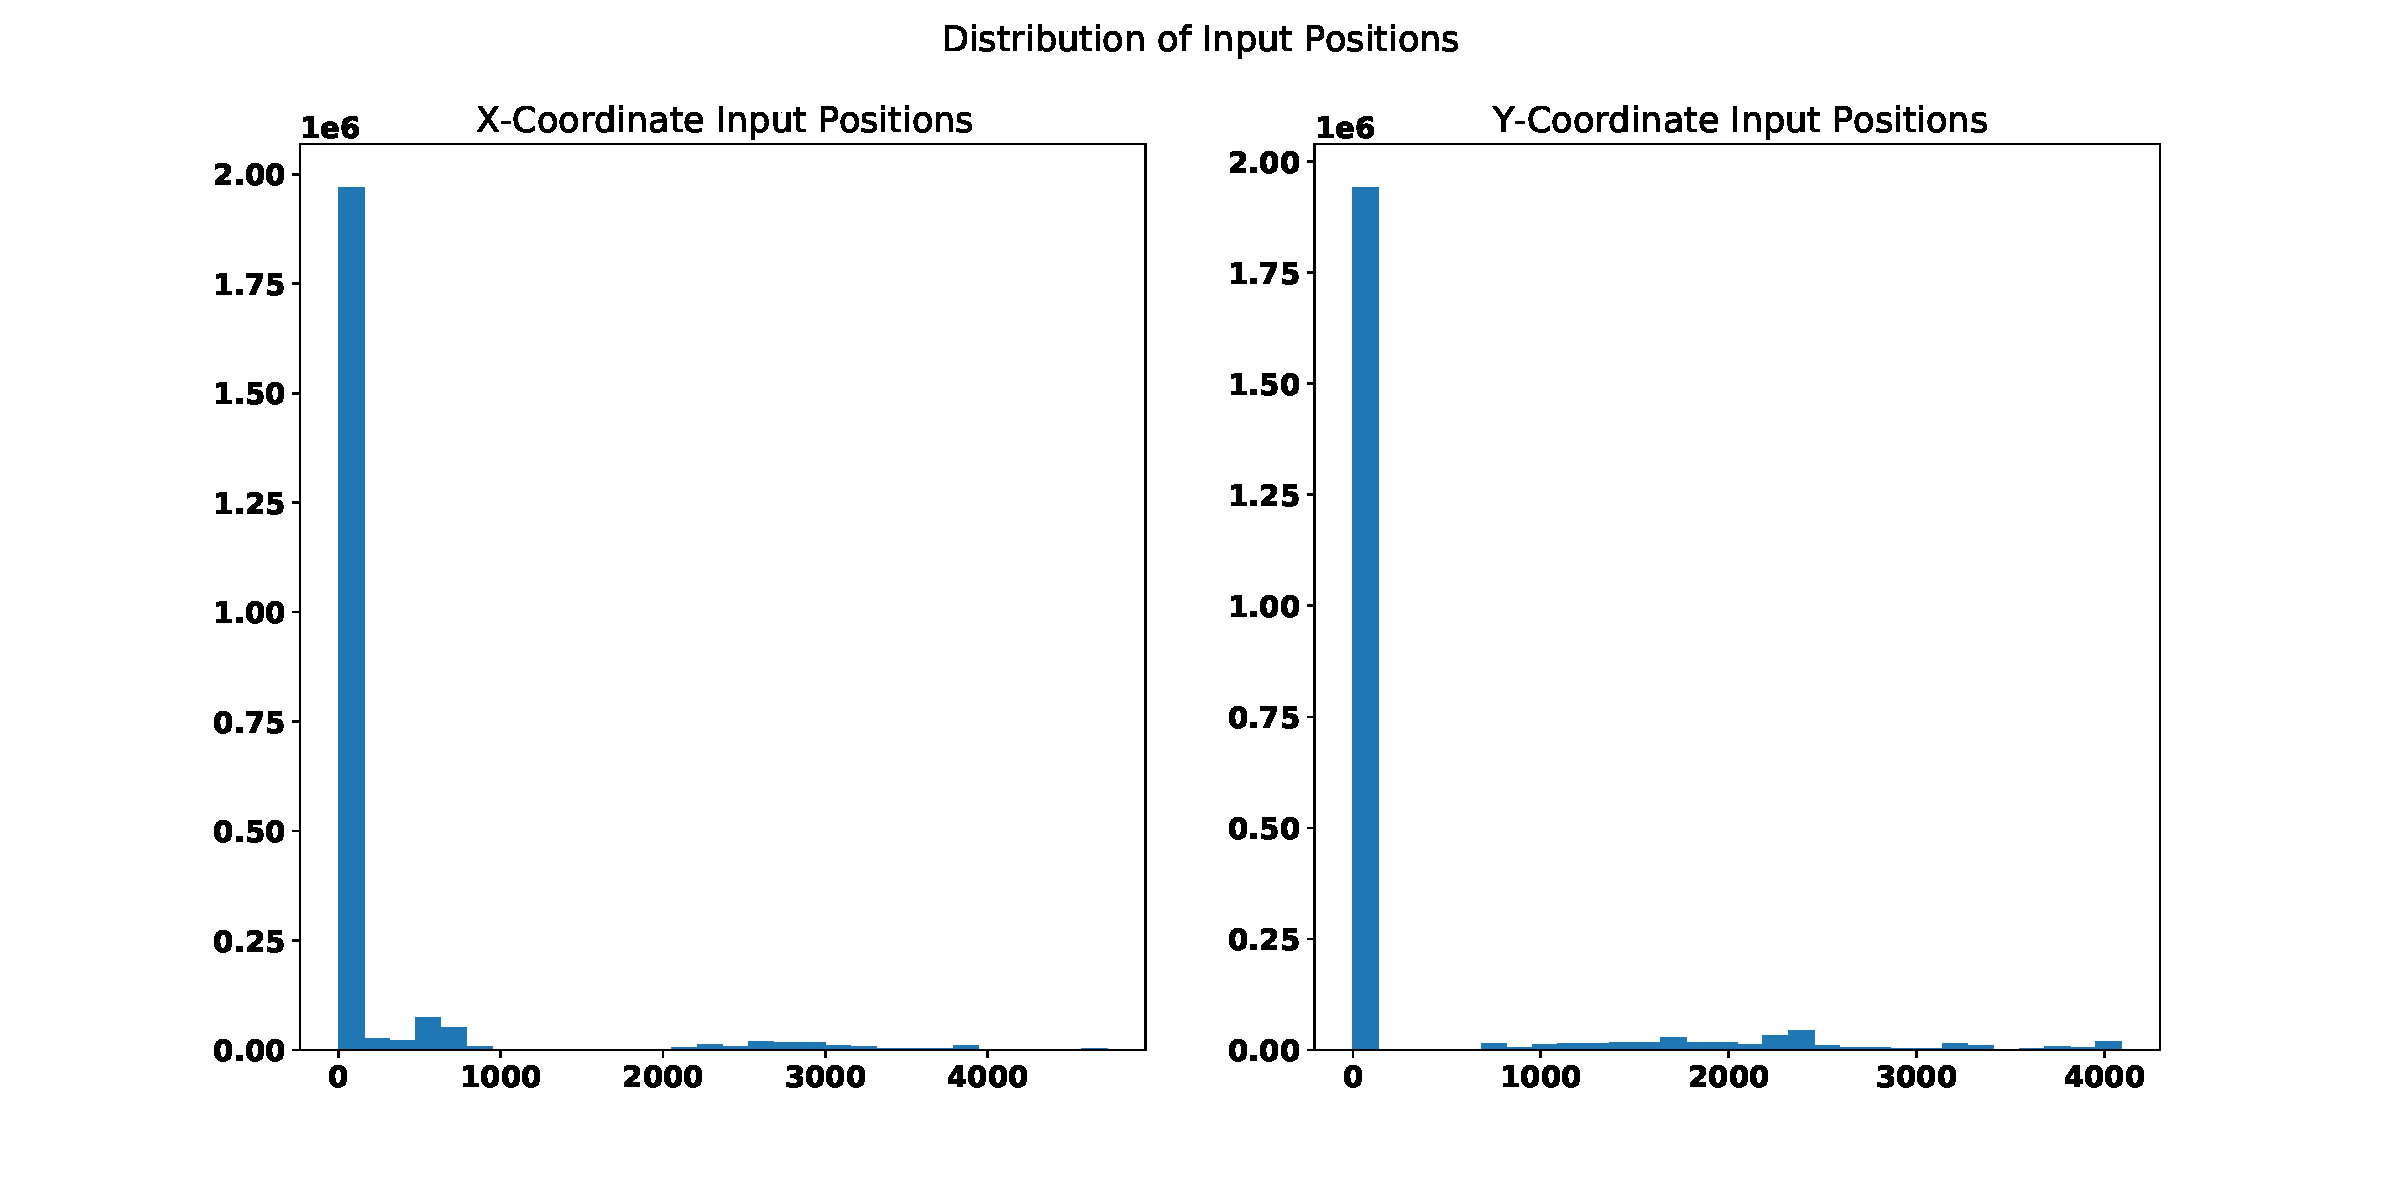
\includegraphics[height=6cm]{figures/sample-in-position-hist.pdf}%
            \caption{Histogram of the X and Y input positions from a subsample of 2000 training files}%
            \label{fig:1}
        \end{figure}        
                
        \begin{figure}[H]
            \centering
            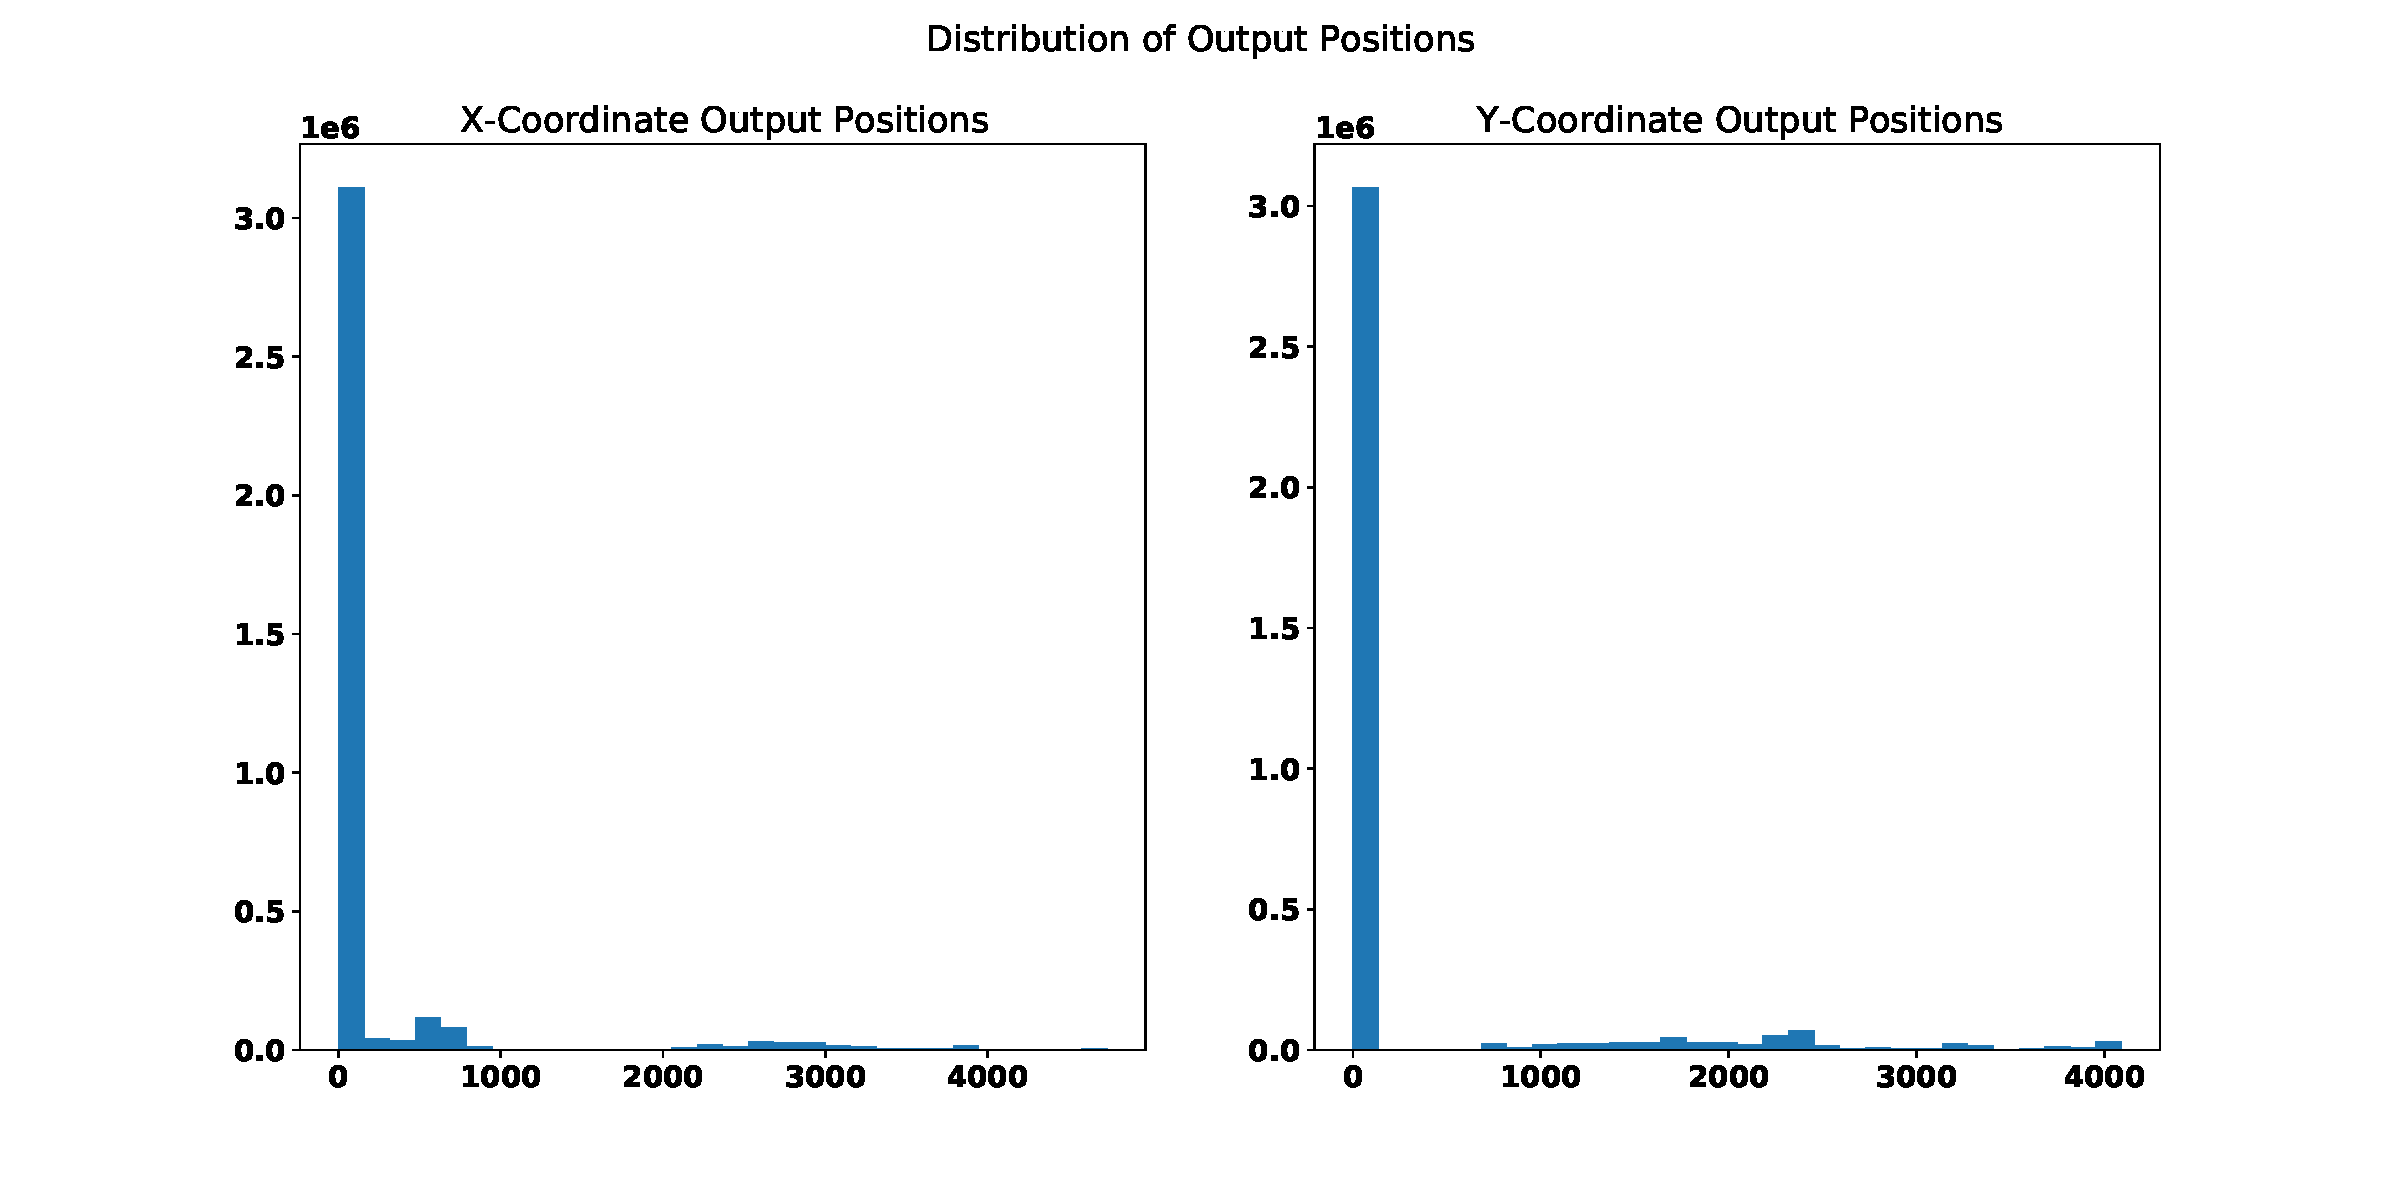
\includegraphics[height=6cm]{figures/sample-out-position-hist.pdf}%
            \caption{Histogram of the X and Y output positions from a subsample of 2000 training files}%
            \label{fig:2}
        \end{figure}

        Analyzing these inputs we find that the vast majority of $(x,y)$ input and output positions are at position $0$, as seen in 
        \autoref{fig:1}, \autoref{fig:2}, and \autoref{table:1} above. Interestingly, the $x$-positions seem to be 
        more closely clustered around $0$, while the $y$-positions 
        have more variance, meaning that most cars are moving mostly in the $y$-dimension, with less overall travel in the $x$-dimension. This
        trend carries through the beginnning and end of the scene (the input and output data).
        
        Looking at only the magnitudes of velocities shows the same trend, with the vast majority of velocities being
        0, however there is also slightly more variance in the distribution of velocties in the $y$-dimension compared to 
        the $x$-dimension.

       
        \begin{figure}[H]
            \centering
            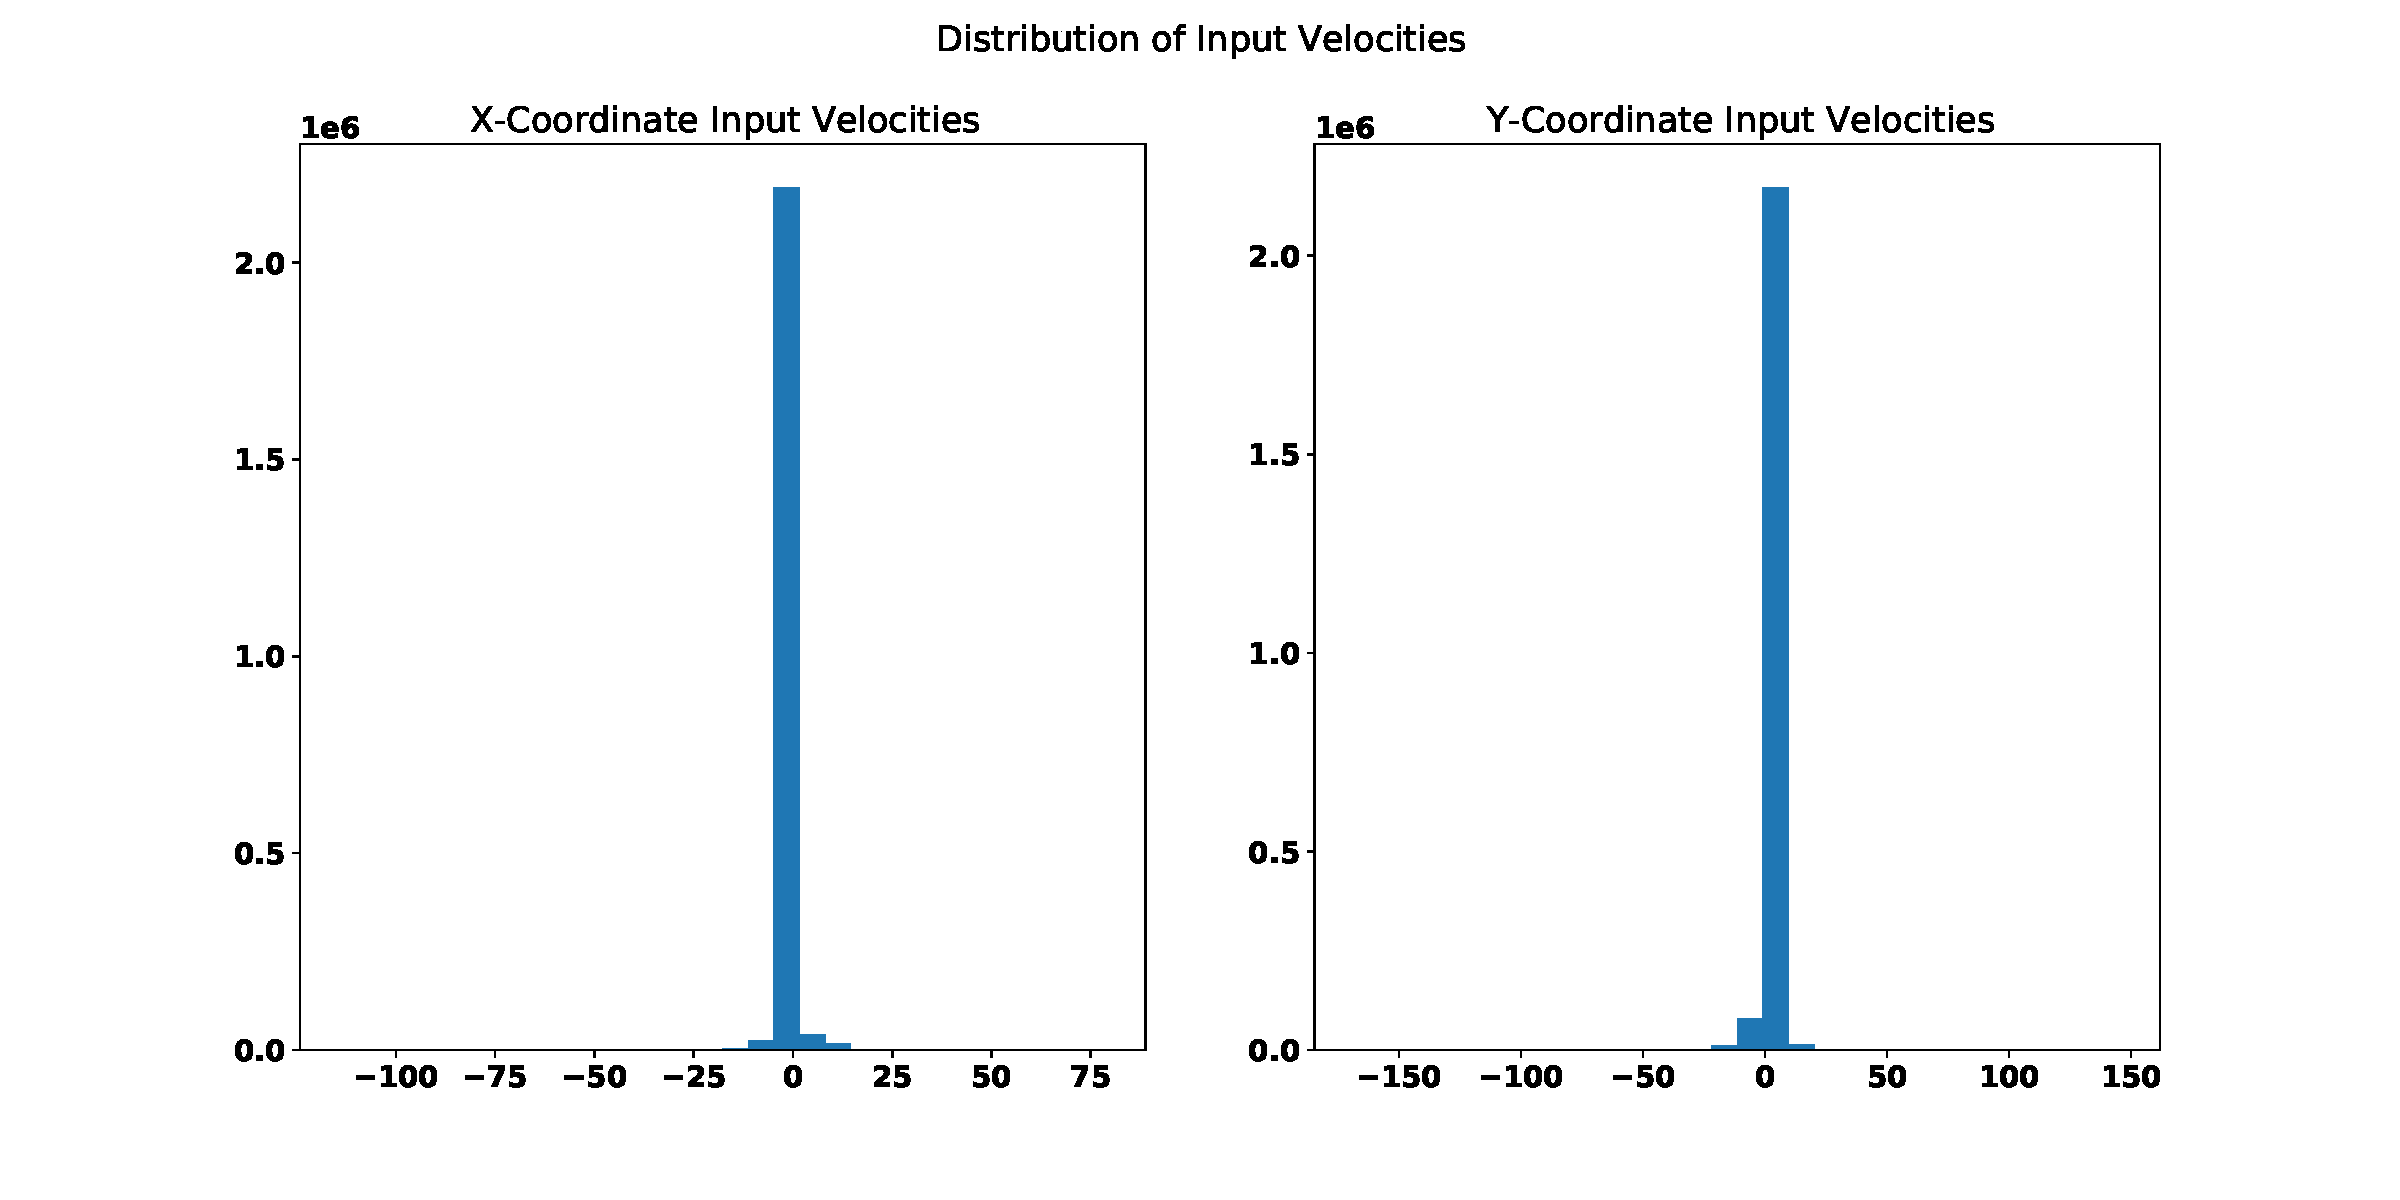
\includegraphics[height=6cm]{figures/sample-in-velocity-hist.pdf}%
            \caption{Histogram of the X and Y input velocities from a subsample of 2000 training files}%
            \label{fig:3}
        \end{figure}
        
        \begin{figure}[H]
            \centering
            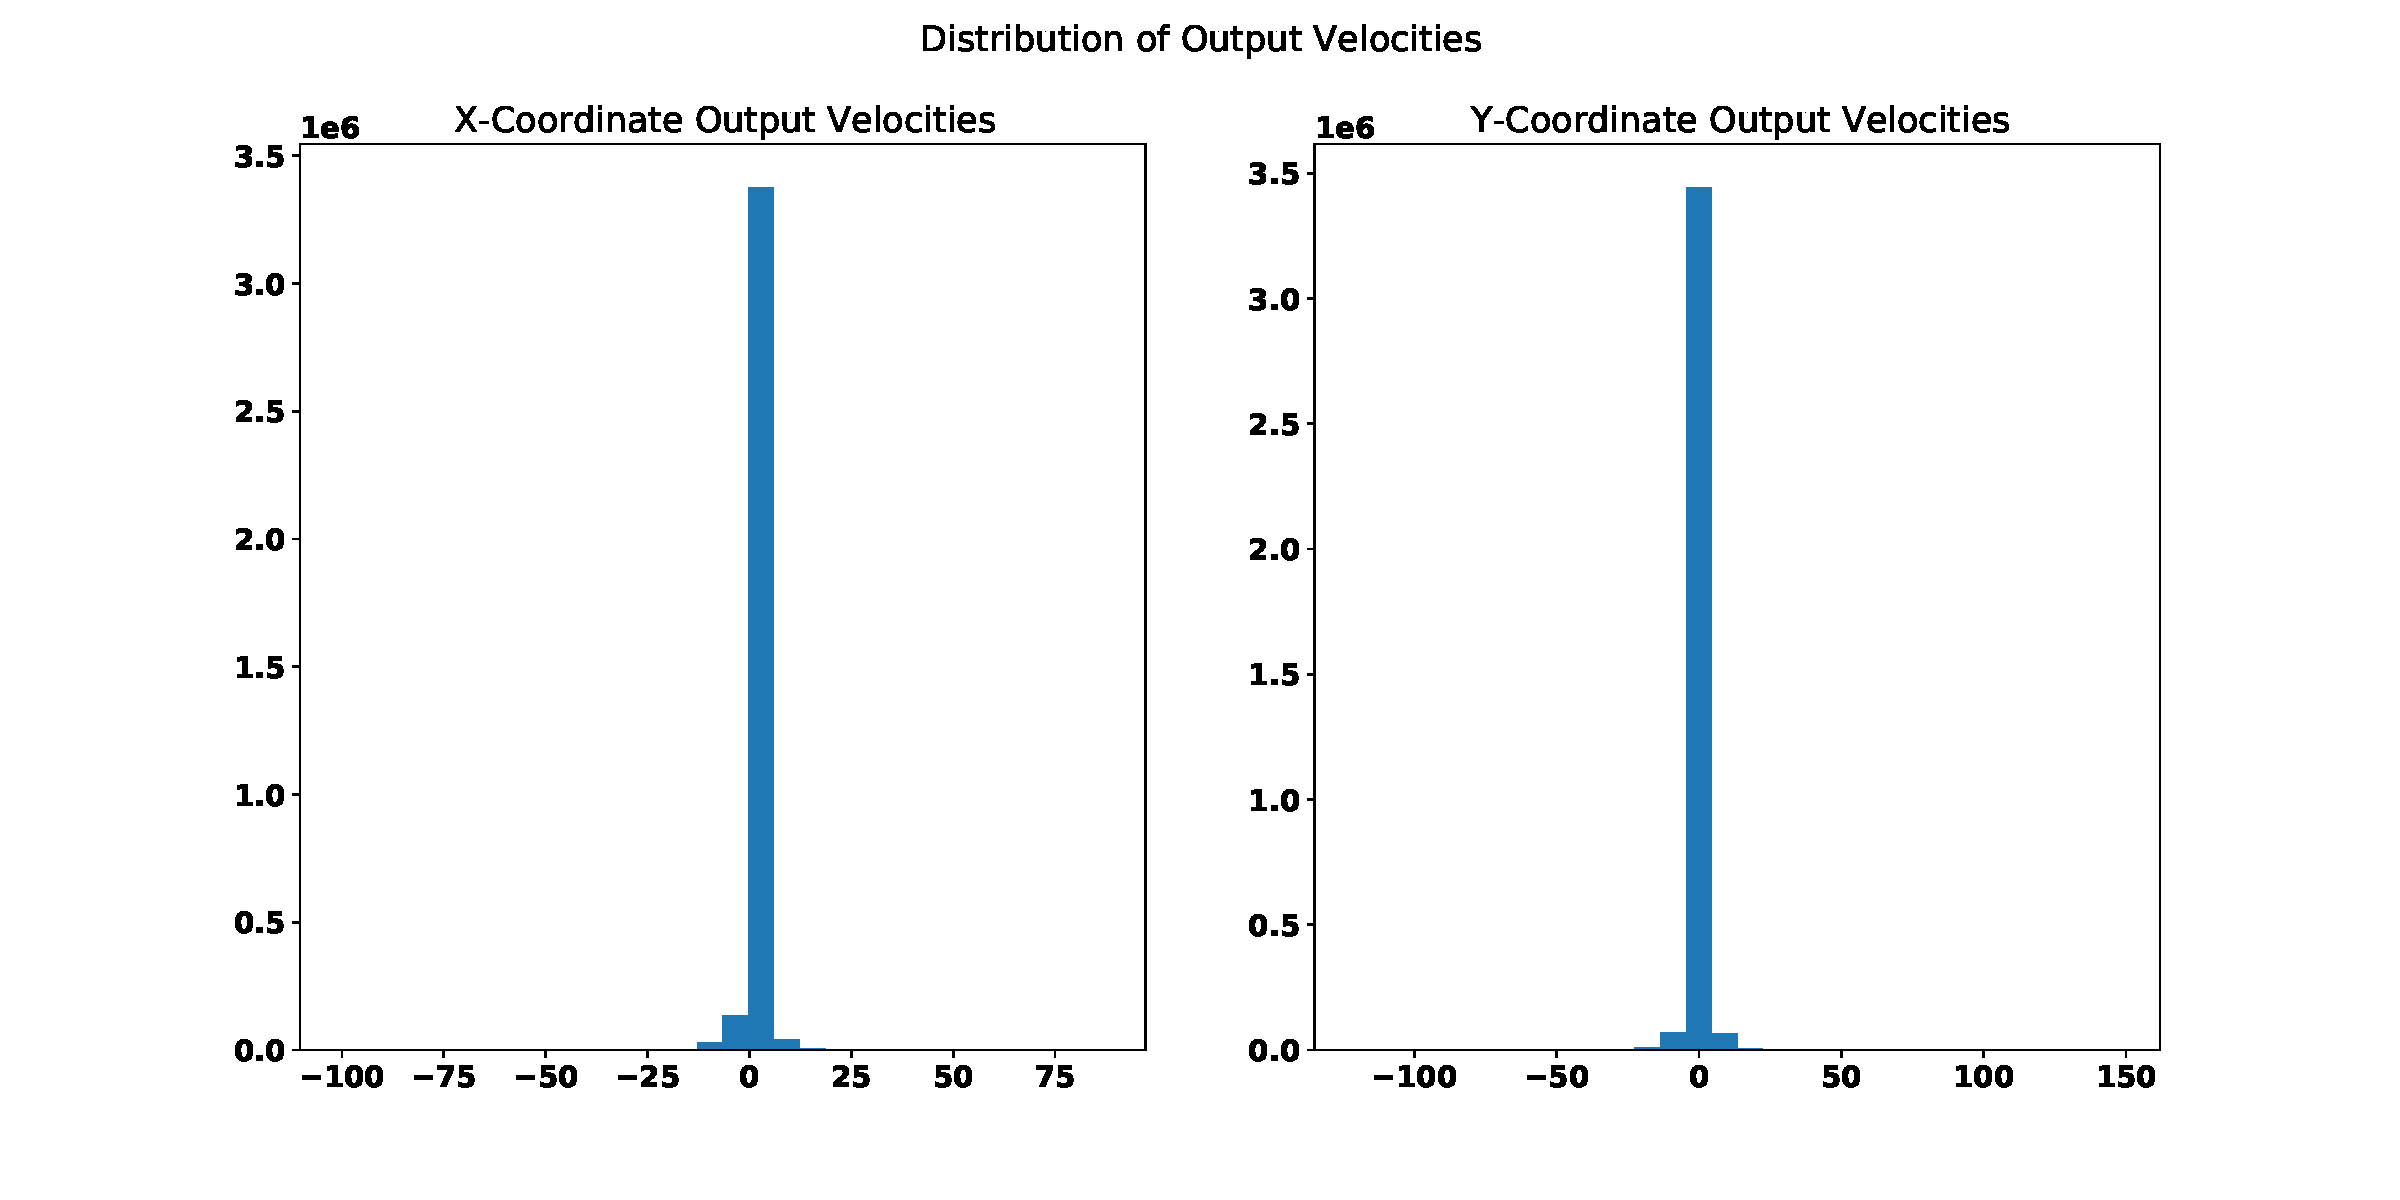
\includegraphics[height=6cm]{figures/sample-out-velocity-hist.pdf}%
            \caption{Histogram of the X and Y output velocities from a subsample of 2000 training files}%
            \label{fig:4}
        \end{figure}

        Taking at a look at the velocity distributions in \autoref{fig:3}, \autoref{fig:4}), annd \autoref{table:2} we again see that the velocities are centered around $0$ in both the $x$ and $y$ dimensions
        at both the beginning and end of each scene. Unlike the position distribution however, velocities can be negative, which is 
        why the distribution is balanced on both sides.
            

\section{Deep Learning Model and Experiment Design}
\label{gen_inst}
    \subsection{Problem A [1 Points]}
        Thus far my best performing model is a PyTorch linear neural net running in an Anaconda environment.
        The platform I am currently working in is my local machine running Ubuntu 20.04 with a 4-core 4-thread Intel i7-7600k CPU 
        running at 4.2 GHz, a GTX 1070 GPU with a max clock speed of 1721 MHz and 8 GB of GDDR5 memory, and 16 GB of 3000 MHz DDR4 memory.
        
        For my initial baseline model I made a simple single layer linear neural network, using Adam as an optimizer And
        and mean square error as my loss function. I used a learning rate of 0.001, and  trained my best model for
        10 epochs. Each epoch took approximately 3 minutes to train.

        I chose mean square error as it increases the penalty for worse predictions, compared to a optimizer like
        mean absolute error, which penalizes with a linear rate. 
        
        In order to get the correct outputs from my trained model, I sliced the output prediction tensors so as to only
        keep the first inner 2 elements of each tensor (the predicted x and y coordinates), and then selected the correct car based on
        each inputs  {\fontfamily{qcr}\selectfont agent\_id}.

    \subsection{Problem B [1 Points]}        

        I experimented with multilayer linear models and an LSTM model as well, however these actually performed worse on 
        the validation set once I uploaded them to Kaggle. Thus far, the best performing model is a linear one, which
        takes in the assumption that cars will be moving at about the same rate over the 5 seconds period of training and prediction.


\section{Experiment Results and Future Work}
\label{headings}
    \subsection{Problem A [1 points]}
        
        \begin{figure}[H]
            \centering
            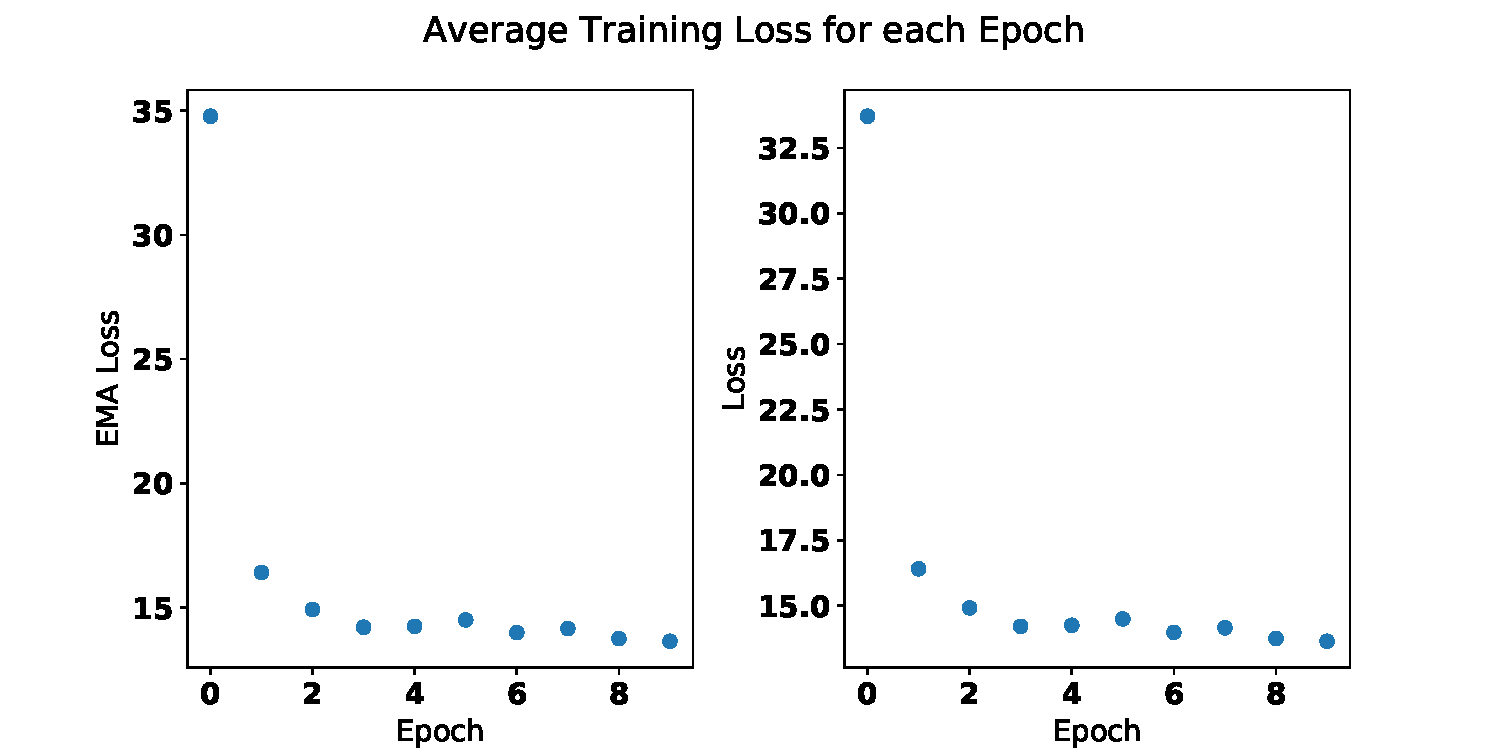
\includegraphics[height=6cm]{figures/train-loss/2021.05.24-multi-linear-ema075-epoch10-batchsz128-epoch-avg.pdf}%
            \caption{Plot of the average training mean square error for my best perfoming single layer model}%
            \label{fig:5}
        \end{figure}

        This model however achieved a significantly lower loss on the training set compared to the final validation set on Kaggle,
        suggesting that my model has overfit the training data. This means that a more complex model with more variance will need to be implemented.

        Based on my lack of success with an LSTM approach, I will continue to work on more complex linear models, as well as trying other architetures
        such as a RNN model, which may achieve a better result as it can take into account previous training examples.

        My current rank on the Kaggle leaderboard is 40 out of 57.

    \appendix

        \section{Appendix}
        
        \url{https://github.com/apfriend/cse151b-kaggle.git}

\end{document}

